\section{Linear Discriminant Analysis}

\begin{frame}
\frametitle{Contents}
\begin{itemize}
\item \important{Introduction to LDA: as a classifier, and as a feature extractor}
\item Introduction to masking countermeasure and Kernel Discriminant Analysis as a feature extractor
\item Motivations to apply deep learning techniques
\item Convolutional Neural Networks and Data Augmentation to attack jitter-based countermeasure
\end{itemize}
\end{frame}


\begin{frame}
\frametitle{Model-based SNR and Fisher's Criterion}
Fisher's criterion for dimensionality reduction is maximize the extracted features SNR
\end{frame}

\begin{frame}
\frametitle{LDA: an optimal linear classifier}
linear separability and
derivation de LDA des modeles generatives (avec hypothese gaussienne et homoscedaticite)
\end{frame}

\begin{frame}
\frametitle{LDA and Fisher's Discriminant}
equivalence under conditions, but conditions not required to apply fisher's discriminant (SCA literature's application of LDA)
\end{frame}

%\begin{frame}
%\frametitle{Projecting Extractors: PCA and LDA}
%\begin{figure}
%\centering{
%\resizebox{11cm}{!}
%{
%\begin{tikzpicture}[remember picture,
%    scale=0.50,
%    % Define styles here
%    every node/.style={transform shape}
%    block/.style={
%        rectangle,
%        draw,
%        text centered,
%        rounded corners
%        },
%    data/.style={
%        trapezium,
%        trapezium left angle=60,
%        trapezium right angle=120,
%        draw
%        },
%    component/.style={
%        circle,
%        draw
%        },
%    output/.style={
%        tape,
%        tape bend top=none,
%        draw
%        },
%    edge/.style={
%        ->,
%        >=stealth,
%        thick
%        }
%    ]
%
%    % Place nodes
%    \node[inner sep=0pt] (genericTrace) at (0,-0)
%    {\includegraphics[width=0.8\textwidth]{figures/genericTrace.pdf} };
%    \node [above=0.1cm of genericTrace] {Rough Trace};
%    \node [block, below left=0.8cm of genericTrace] (PCA) {\begin{Large}PCA\end{Large}};
%    \node [block, below right=0.8cm of genericTrace] (LDA) {\begin{Large}LDA\end{Large}};
%    \node [below=1.5cm of genericTrace](puntini) {\begin{Large}$\dots$\end{Large}};
%    \node [component, left=0.5cm of puntini](PC2) {\begin{Large}$\AAlpha_2$\end{Large}};
%    \node [component, left=0.5cm of PC2](PC1) {\begin{Large}$\AAlpha_1$\end{Large}};
%    \node [component, right=0.25cm of puntini](PCC) {\begin{Large}$\AAlpha_C$\end{Large}};
%   \node [right=0.25cm of PCC](puntini2) {\begin{Large}$\dots$\end{Large}};
%    \node [component, right=0.15cm of puntini2](PCr) {\begin{Large}$\AAlpha_r$\end{Large}};
%    %\draw[thick, black,decorate,decoration={brace,amplitude=10pt}](PC1.north) -- (PCr.north);
%    \draw(PC1.north)  to [bend left=15] (PCr.north);
%    
%    
%    \draw[->, shorten >=20pt] (PCA.north) node[above=0.4cm] {Principal Components (PCs)} to [bend left] (PC2.north) ;
%     \draw[->,shorten >=25pt] (LDA.north)  node[above=0.35cm] {Discriminant Components (DCs)} to [bend right] (puntini2.north);
%     
%    \only<2>{ 
%    \node [data, below=1cm of puntini](formula1) {\begin{Large}$\sum_{j=1}^D\AAlpha_1[j]\textbf{x}[j]$\end{Large}};
%    \node [left=0.5cm of formula1] {Linear Combination / Projection};
%    \node [below=0.5cm of formula1] (compressed1)
%    	{\includegraphics[width=0.5\textwidth]{figures/compressed1.pdf} }; 
%    	\node[right=0.1cm of compressed1]{Reduced Trace}; 
%	\draw[-, red, thick, shorten >=6pt, shorten <=-6pt](genericTrace.south) to (PC1.north);
%	\draw[-, red, thick, shorten >=6pt, shorten <= 6pt](PC1.south) to (formula1.north);
%	\draw[-, red, thick, shorten <= 2pt, shorten >=-5pt](formula1.south) to (compressed1.north);
%}
%    
%        \only<3>{ 
%        \node [data, below=1cm of puntini](formula2) {\begin{Large}$\sum_{j=1}^D\AAlpha_2[j]\textbf{x}				[j]$\end{Large}};
%    \node [left=0.5cm of formula2] {Linear Combination / Projection};
%    \node [below=0.5cm of formula2] (compressed2)
%    	{\includegraphics[width=0.5\textwidth]{figures/compressed2.pdf} };  
%    	\node[right=0.1cm of compressed2]{Reduced Trace};
%	\draw[-, red, thick, shorten >=6pt, shorten <=-6pt](genericTrace.south) to (PC2.north);
%	\draw[-, red, thick, shorten >=6pt, shorten <= 6pt](PC2.south) to (formula1.north);
%	\draw[-, red, thick, shorten <= 2pt, shorten >=-5pt](formula2.south) to (compressed2.north);
%}
%
% \uncover<4>{ 
%        \node [data, below=1cm of puntini](formulaC) {\begin{Large}$\sum_{j=1}^D\AAlpha_C[j]\textbf{x}				[j]$\end{Large}};
%    \node [left=0.5cm of formulaC] {Linear Combination / Projection};
%    \node [below=0.5cm of formulaC] (compressedC)
%    	{\includegraphics[width=0.5\textwidth]{figures/compressedAll.pdf} }; 
%    \node[right=0.1cm of compressedC]{Reduced Trace};
%	\draw[-, red, thick, shorten >=6pt, shorten <=-6pt](genericTrace.south) to (PCC.north);
%	\draw[-, red, thick, shorten >=6pt, shorten <= 6pt](PCC.south) to (formulaC.north);
%	\draw[-, red, thick, shorten <= 2pt, shorten >=-5pt](formulaC.south) to (compressedC.north);
%}
%    
%     
%     
%
%\end{tikzpicture}
%}
%}
%
%\end{figure}
%\end{frame}



\begin{frame}
\frametitle{PCA and LDA}
\only<1>{
\vspace{-50pt}
\begin{block}{Standard PCA}
\begin{itemize}
\item maximizing data variance
\item not exploiting sensitive variable knowledge
\end{itemize}
\end{block}
\vfill
}
\only<2->{
\begin{block}{Class-oriented PCA}
\begin{itemize}
\item\only<2->{eigenvector research}
\item \only<2->{maximizing inter-class variance}
\item \only<3->{not minimizing the intra-class variance}
\item \only<4->{easily and accurately computable (no matrix inversions)}
\item \only<5->{\textcolor{red}{components selection issue} (disagreement between theory and experience)$\longrightarrow $ ELV selection tool [CARDIS 2015]}
\end{itemize}
\end{block}
}
\only<2-5>{
\begin{block}{LDA}
\begin{itemize}
\item\only<2-5>{eigenvector research}
\item \only<2-5>{maximizing inter-class variance while minimizing intra-class variance (no loss of information under some leakage model \cite{lessIsMore})}
\item \only<4-5> {not easily computable (asking for a matrix inversion)}
\end{itemize}
\end{block}
}



\end{frame}

\begin{frame}
\frametitle{Overview of experimental results of the ELV selection tool}
\begin{block}{Overview of experimental results of the ELV selection tool}
\begin{itemize}
\item large profiling set: PCA performances close to the LDA's if equipped with ELV (and less expensive)
\item small profiling set: LDA efficiency decreases faster than (PCA $+$ ELV)'s \item too small profiling set: LDA unavailable. PCA$+$ELV still efficient
\end{itemize}

\end{block}
\end{frame}

%\subsubsection{Components Selection Issue}
%
%\begin{frame} \frametitle{The Problem of Selecting PCA Components}
%
%% state of the art
%% first and sixth PC DPA contest
%\begin{columns}
%\begin{column}{0.1\textwidth}
%\includegraphics[width = \textwidth]{figures/questionmark.jpg} 
%\end{column}
%\begin{column}{0.7\textwidth}
%\begin{block}{}
%{\em How many} PCs and {\em which ones} are sufficient/necessary to reduce the traces size without losing important discriminant information?
%\end{block}
%\end{column}
%\end{columns}
%\vspace{-7pt}
%\begin{block}{Experimental Observation}
%\cite{Batina2012,specht}: the first components sometimes contain no sensitive information; it is worth discarding them.
%\end{block}
%\begin{figure}
%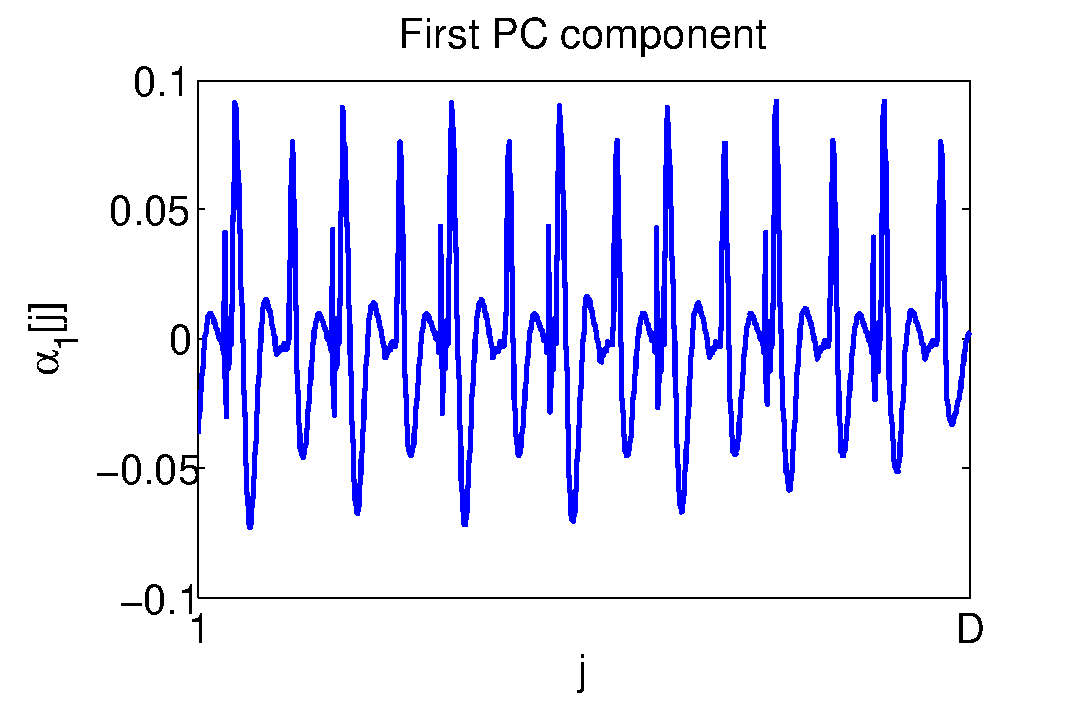
\includegraphics[width=.45\textwidth]{figures/DPAcontestPC1_new.pdf} 
%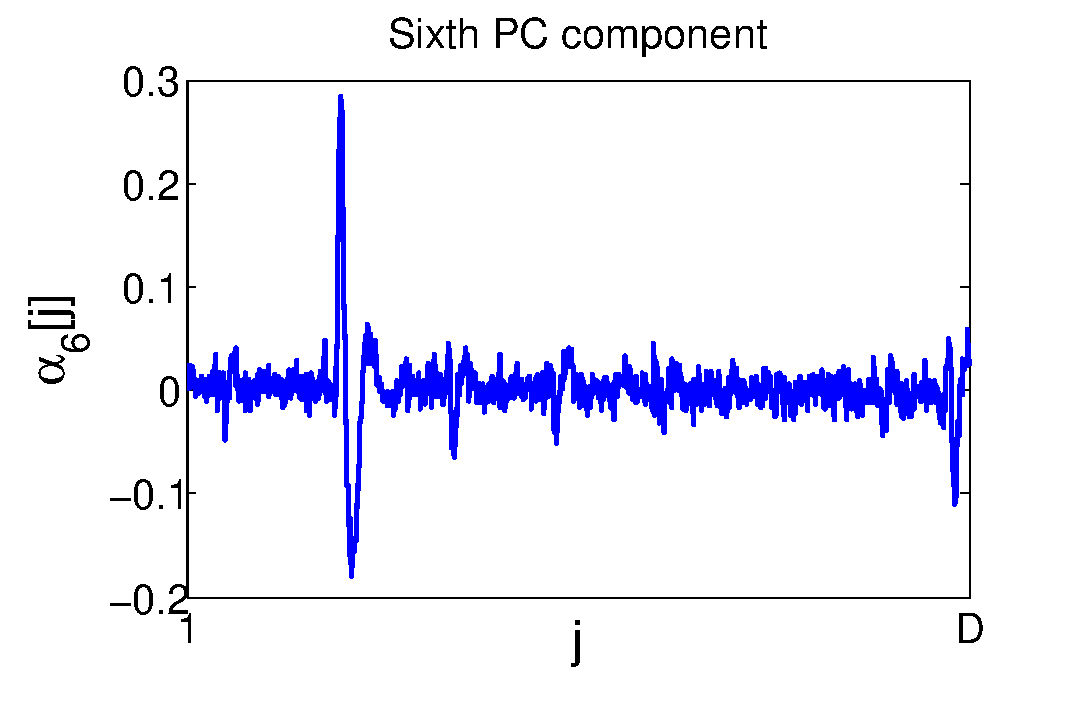
\includegraphics[width=.45\textwidth]{figures/DPAcontestPC6_new.pdf} 
%\caption{First and sixth PCs in DPA contest v4  \cite{DPAcontest} trace set}\label{fig:DPAcontest}
%\end{figure}
%
%
%
%
%
%\end{frame}
%
%
%\begin{frame} \frametitle{The Problem of Selecting PCA Components - EGV, IPR}
%\begin{block}{Explained Global Variance (EGV)}
%$\EGV{\AAlpha_i} = \frac{\lambda_i}{\sum_{k=1}^r \lambda_k}$\\
%\cite{choudaryefficient} : 
%\begin{itemize}
%\item fix a threshold $\beta$
%\item choose the first $C$ components, where $C$ is the minimum integer such that
%\begin{equation*}
%\EGV{\AAlpha_1}+ \EGV{\AAlpha_2}+\dots + \EGV{\AAlpha_C} \geq \beta
%\end{equation*}
%\end{itemize}
%\end{block}
%%\begin{block}{Assumption}
%%Dealing with secured devices, the leaking side-channel information is localised in few points of the acquired trace.
%%\end{block}
%
%\begin{block}{Inverse Participation Ratio (IPR)}
%\cite{SCAclassProbl}: 
%\begin{equation*}
%\mathrm{IPR}(\AAlpha_i) = \sum_{j=1}^\traceLength \AAlpha_i[j]^4 \mbox{ \em (localization score)}
%\end{equation*}
%\end{block}
%\end{frame}


%\begin{frame} \frametitle{The Component Selection Issue}
%
%\begin{columns}
%\begin{column}{0.1\textwidth}
%\includegraphics[width = \textwidth]{figures/questionmark.jpg} 
%\end{column}
%\begin{column}{0.7\textwidth}
%\begin{block}{}
%{\em How many} PCs and {\em which ones} are sufficient/necessary to reduce the traces size without losing important discriminant information? 
%\end{block}
%\end{column}
%\end{columns}
% \only<1>{
% \begin{block}{Theoretically}
%Higher eigenvalues $\longrightarrow$ higher information.
%\end{block}
%\begin{block}{Experimental Observation}
%\cite{Batina2012,specht}: the first components sometimes contain no sensitive information; it is worth discarding them.
%\end{block}
%
%\begin{figure}
%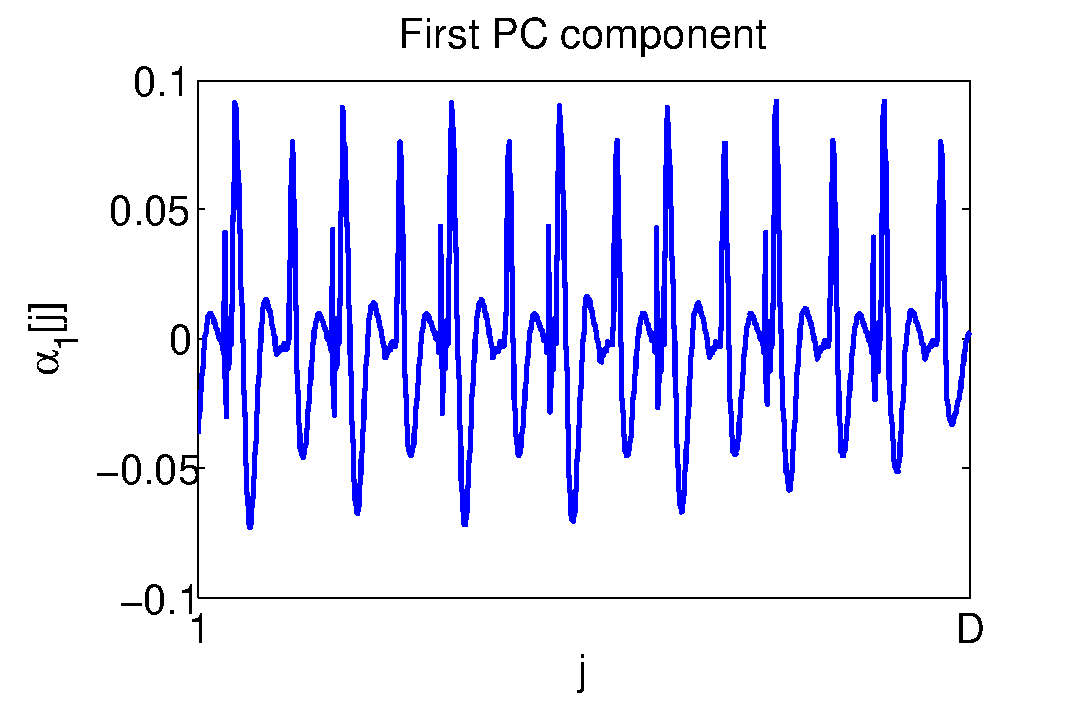
\includegraphics[width=.25\textwidth]{figures/DPAcontestPC1_new.pdf} 
%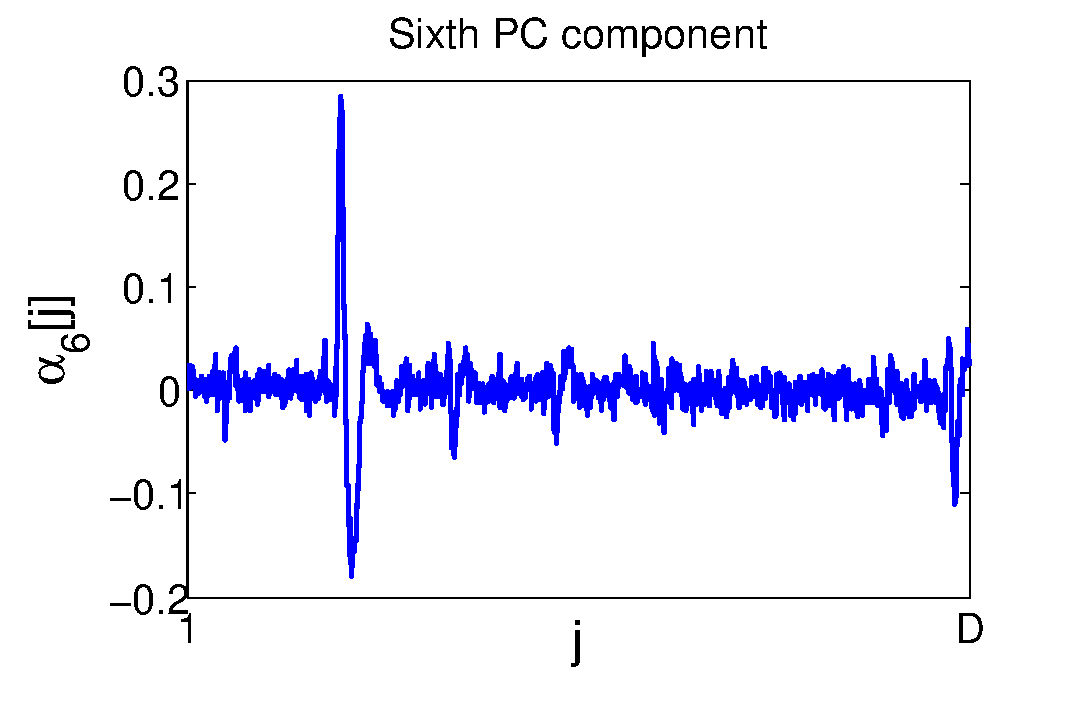
\includegraphics[width=.25\textwidth]{figures/DPAcontestPC6_new.pdf} 
%\vspace{-10pt}
%\caption{First and sixth PCs in DPA contest v4  \cite{DPAcontest} trace set}\label{fig:DPAcontest}
%\end{figure}
%}
%\only<2>{
%\vspace{40pt}
%\begin{small}
%\begin{table}
%\begin{tabular}{|c|c|c|c|}
%\hline
%& EGV \cite{choudaryefficient} & IPR \cite{SCAclassProbl}& \uncover<2->{\textbf{ELV} \cite{Cagli2016}} \\
%\hline
%eigenvalue $\lambda_i$ &
\includegraphics[scale=0.01]{figures/yes.png}  & 
\includegraphics[scale=0.01]{figures/no.png} &\uncover<2->{
\includegraphics[scale=0.015]{figures/yes.png}}\\
%\hline
%form of $\AAlpha_i$ &
\includegraphics[scale=0.01]{figures/no.png}  & 
\includegraphics[scale=0.01]{figures/yes.png}&\uncover<2->{
\includegraphics[scale=0.015]{figures/yes.png}} \\
%\hline
%\end{tabular}
%\end{table}
%\end{small}
%
%\includegraphics[scale=0.3]{figures/citazione1.jpg} 
%}
%\uncover<2->{
%\begin{block}{Explained Local Variance}
%$\mathrm{ELV}(\AAlpha_i,j) = \frac{\lambda_i \AAlpha_i[j]^2}{\sum_{k=1}^r\lambda_k} = \mathrm{EGV}(\AAlpha_i) \AAlpha_i[j]^2$  \\
%%($\sum_{j=1}^D \mathrm{ELV}(\AAlpha_i,j) = \EGV{\AAlpha_i}$)
%\end{block}
%}
%\uncover<3->{\begin{block}{Use of the ELV}
%\begin{itemize}
%\item Sort in decreasing order the maximal ELV provided by each component $\{\max_{j=1,\dots,D}\ELV(\AAlpha_i,j)\}_{i}$ and select the $C$ first components.
%\item Select \textbf{couples} $(\AAlpha_i, j)$ in decreasing order wrt to $\ELV(\AAlpha_i, j)$ until $\ELV(\AAlpha_{i_1}, j_1)+ \ELV(\AAlpha_{i_2}, j_2)+\dots +\ELV(\AAlpha_{i_M}, j_M)\geq \beta$
%\end{itemize}
%\end{block}}
%\end{frame}

%\begin{frame} \frametitle{The ELV Selection (2)}
%\vspace*{-0.5cm}
%\uncover<1->{
%\begin{block}{Definition}
%$\mathrm{ELV}(\AAlpha_i,j) = \frac{\lambda_i \AAlpha_i[j]^2}{\sum_{k=1}^r\lambda_k} = \mathrm{EGV}(\AAlpha_i) \AAlpha_i[j]^2$  \\
%\uncover<2->{Observe that $\sum_{j=1}^D \mathrm{ELV}(\AAlpha_i,j) = \EGV{\AAlpha_i}$}
%\end{block}
%}
%\uncover<3->{
%Perform this sum in a cumulative way, sorting the ELV contributions of the time samples in decreasing order, {\em i. e.} $\mathrm{ELV}(\AAlpha_i,j^i_1)\geq \mathrm{ELV}(\AAlpha_i,j^i_2)\geq \dots \geq \mathrm{ELV}(\AAlpha_i,j^i_\traceLength)$
%
%
%\vspace*{-0.4cm}
%\begin{columns}
%\begin{column}{.5\textwidth}
%\vspace*{10pt}
%\begin{figure}
%\includegraphics[width=\textwidth]{figures/PC1_points.pdf} 
%\end{figure}
%\end{column}
%\begin{column}{.5\textwidth}
%\begin{figure}
%
%\begin{tikzpicture}[remember picture,
%    scale=1,
%    % Define styles here
%    every node/.style={transform shape}
%    block/.style={
%        rectangle,
%        draw,
%        text centered,
%        rounded corners
%        },
%    data/.style={
%        trapezium,
%        trapezium left angle=60,
%        trapezium right angle=120,
%        draw
%        },
%    component/.style={
%        circle,
%        draw
%        },
%    output/.style={
%        tape,
%        tape bend top=none,
%        draw
%        },
%    edge/.style={
%        ->,
%        >=stealth,
%        thick
%        }
%    ]
%
%    \node (only1elv) at (0,0)
%    {\includegraphics[width=\textwidth]{figures/cumulativeELV_only1.pdf} };
%    \node [component, thick, xshift=2.1cm, yshift=0.8cm] (cerchio) {};
%    \node[below left=1cm of cerchio](caption){$\mathrm{EGV}(\AAlpha_1)$};
%    \draw[->] (caption) to (cerchio.south west);
%\end{tikzpicture}
%\end{figure}
%\end{column}
%\end{columns}
%
%
%}
%
%\end{frame}



%\begin{frame}
%\frametitle{The ELV Selection (2)}
%\begin{columns}
%\begin{column}{0.5\textwidth}
%\uncover<1->{
%\only<1>{
%\vspace*{-0.4cm}
%\begin{center}
%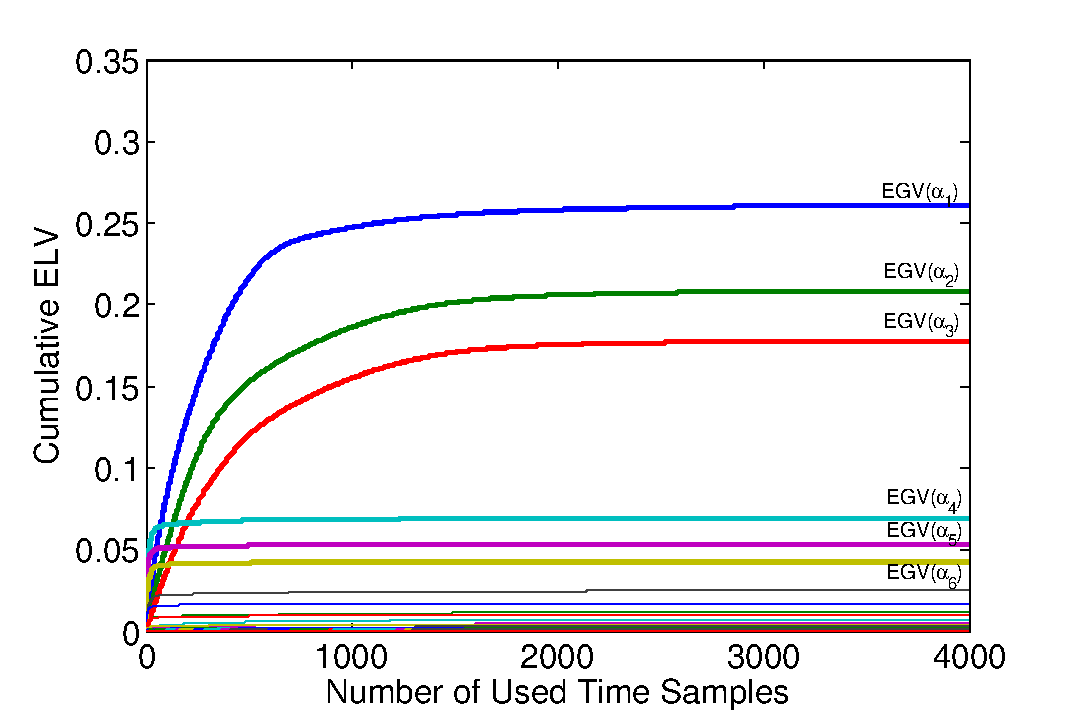
\includegraphics[width = \textwidth]{figures/cumulativeELV.pdf}
%\end{center}
%}
%\only<2>{
%\vspace*{-0.4cm}
%\begin{center}
%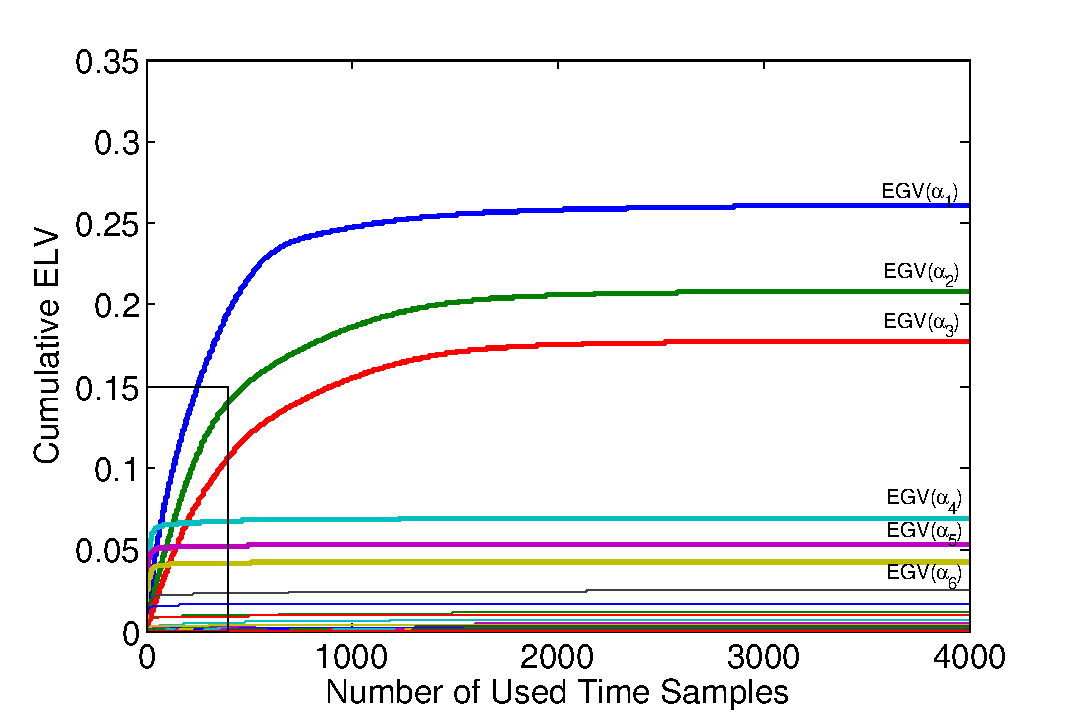
\includegraphics[width = \textwidth]{figures/cumulativeELVallRectangle.pdf} 
%\end{center}
%}
%
%\only<3->{
%\vspace*{-0.4cm}
%\begin{center}
%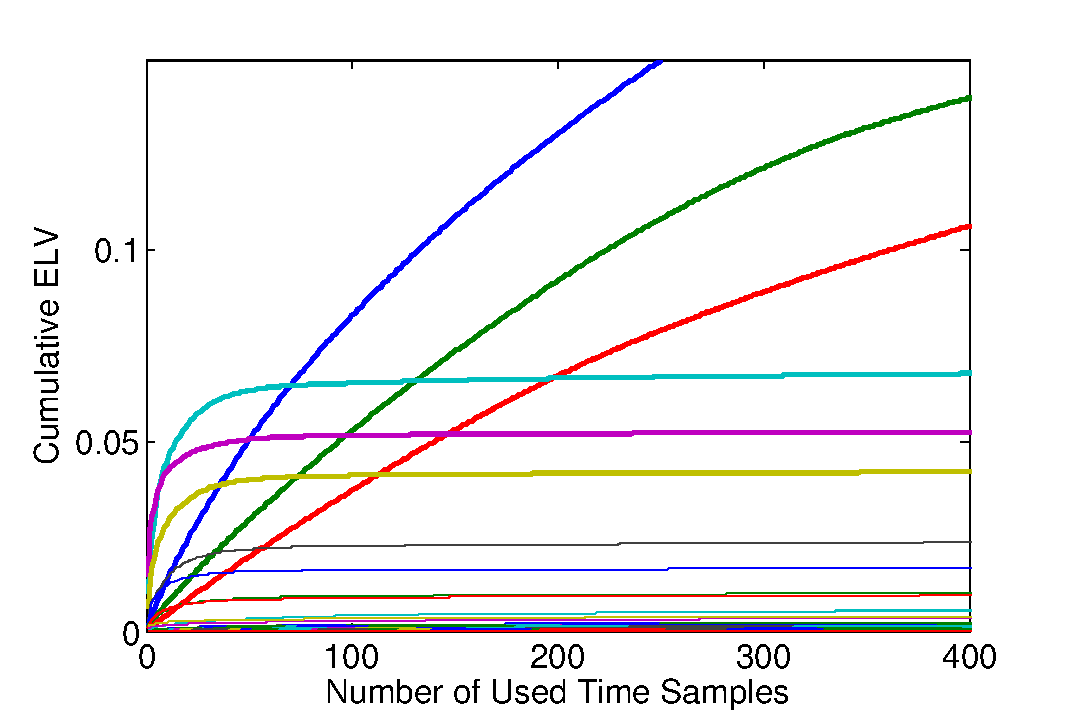
\includegraphics[width = \textwidth]{figures/cumulativeELVzoomed.pdf}
%\end{center}
%}
%}
%\uncover<4->{
%\only<1-4>{
%
%\begin{block}{To select $C$ components\hspace{\textwidth}\textcolor{white}{ }}
%Sort in decreasing order the maximal ELV provided by each component $\{\max_{j=1,\dots,D}\ELV(\AAlpha_i,j)\}_{i}$ and select the $C$ first components.
%\end{block}
%}
%\only<5>{
%
%\begin{block}{Fixing a cumulative explained variance threshold $\beta$}
%Select \textbf{couples} $(\AAlpha_i, j)$ in decreasing order wrt to $\ELV(\AAlpha_i, j)$ until $\ELV(\AAlpha_{i_1}, j_1)+ \ELV(\AAlpha_{i_2}, j_2)+\dots +\ELV(\AAlpha_{i_M}, j_M)\geq \beta$.\\
%%\uncover<5>{{\em Components denoising}}
%\end{block}
%}
%}
%
%\end{column}
%
%\begin{column}{0.5\textwidth}
%\only<1-3>{
%\begin{figure}
%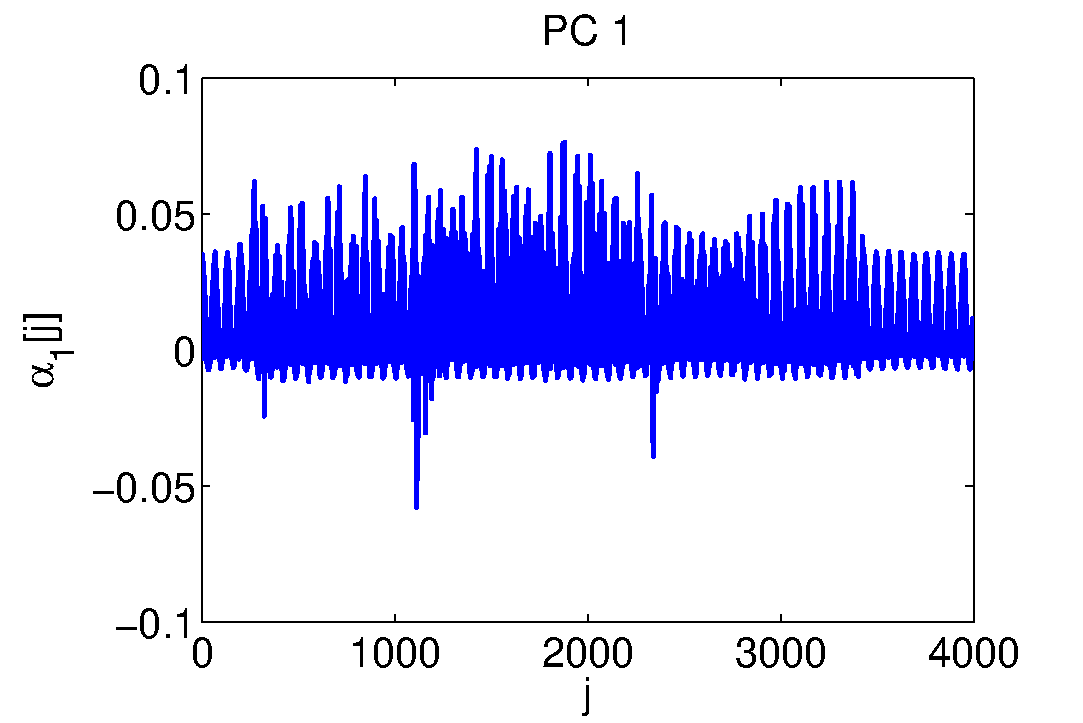
\includegraphics[width=0.5\textwidth]{figures/PC1.pdf} 
%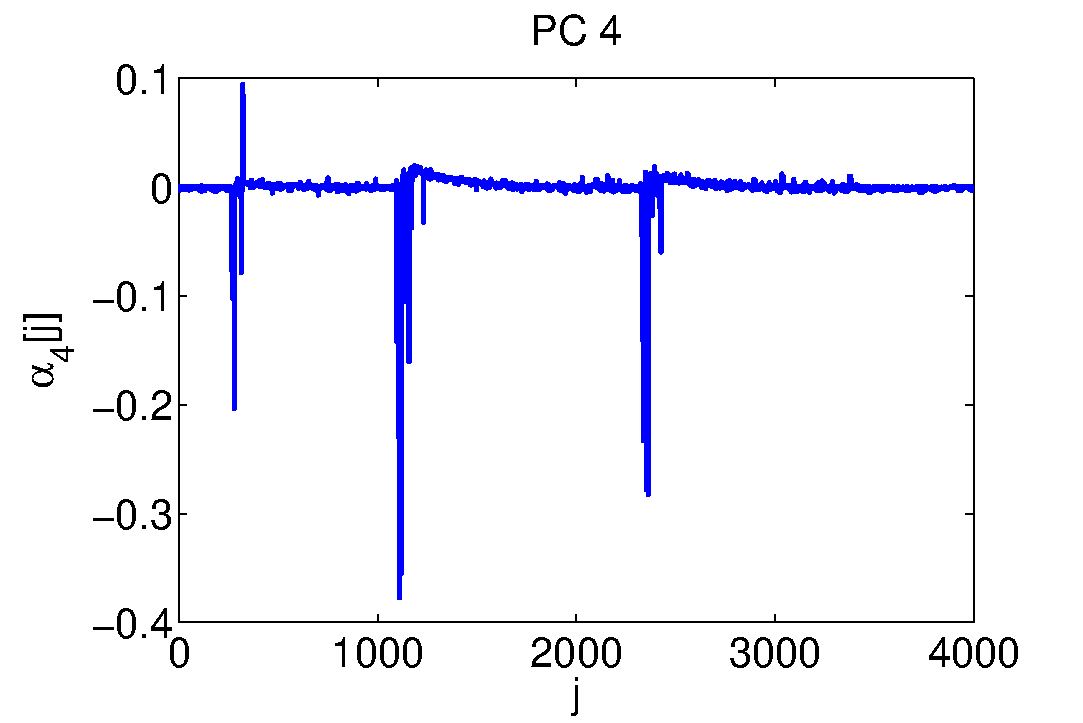
\includegraphics[width=0.5\textwidth]{figures/PC4.pdf} \\
%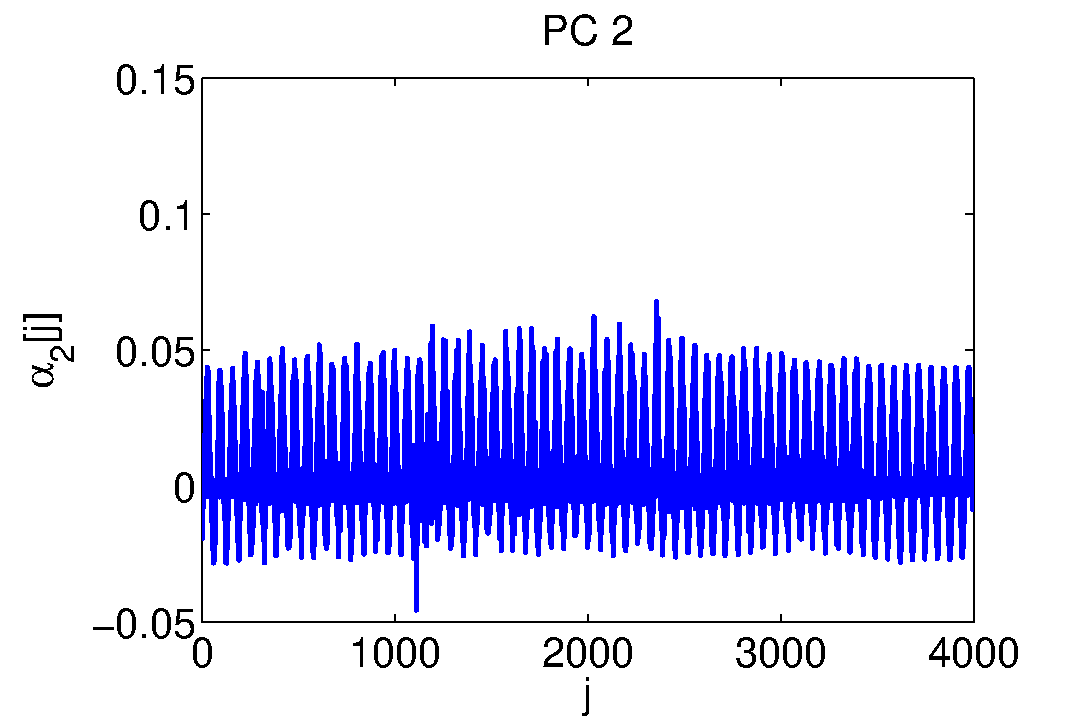
\includegraphics[width=0.5\textwidth]{figures/PC2.pdf} 
%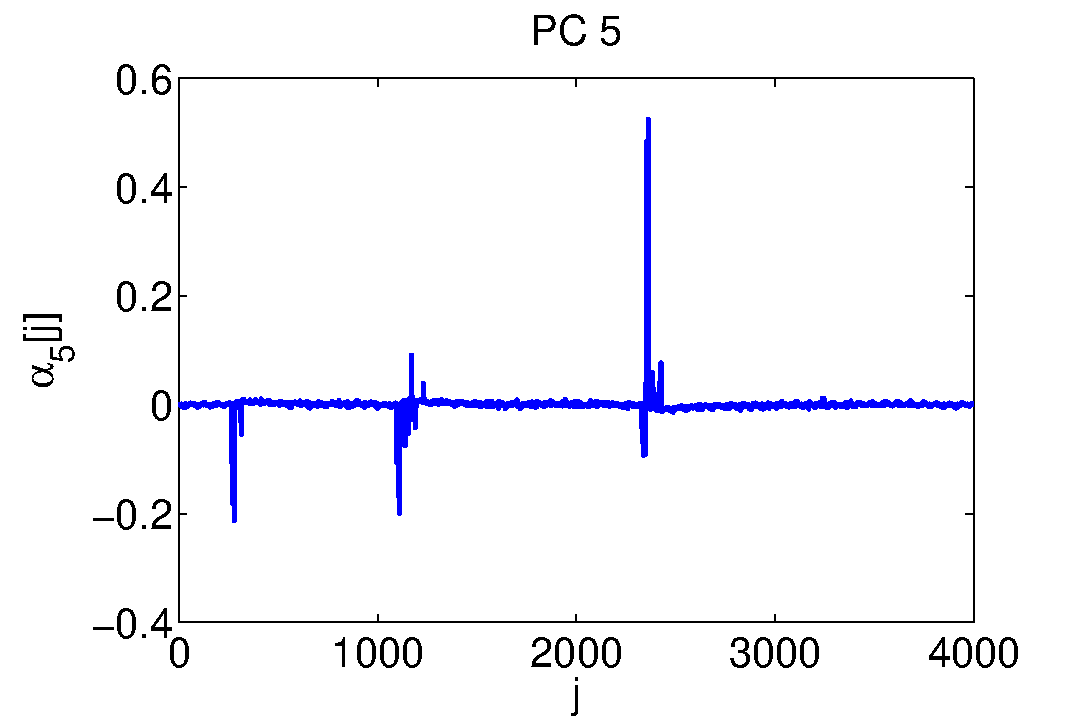
\includegraphics[width=0.5\textwidth]{figures/PC5.pdf} \\
%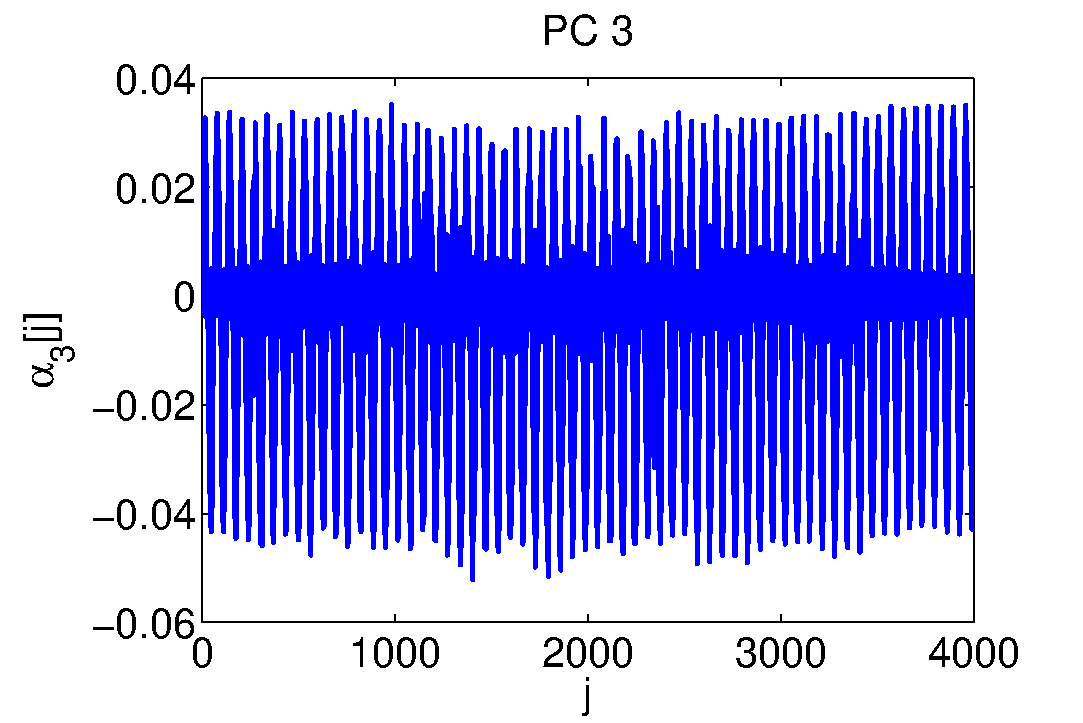
\includegraphics[width=0.5\textwidth]{figures/PC3.pdf} 
%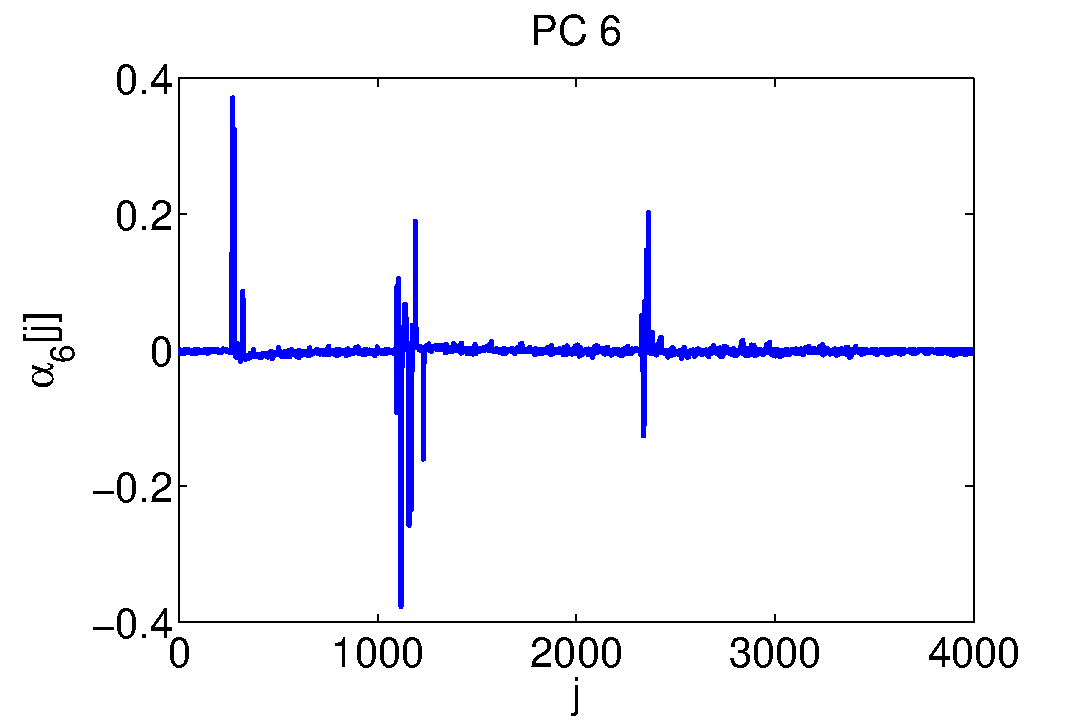
\includegraphics[width=0.5\textwidth]{figures/PC6.pdf} 
%\caption{\begin{footnotesize}
%The first 6 PCs: 
%$\lambda_1 \approx 3.8 ,\lambda_2 \approx 3.1 , \lambda_3 \approx2.6 ,\lambda_4 \approx 1.0 ,\lambda_5 \approx 0.8 ,\lambda_6 \approx 0.6 $
%\end{footnotesize}}
%
%\end{figure}
%}


%\only<4-5>{
%\begin{figure}
%\onslide<5->{\includegraphics[width=0.5\textwidth]{figures/PC5_denoised.pdf}}\only<4>{\includegraphics[width=0.5\textwidth]{figures/PC5_cerchio.pdf}}\only<5>{\includegraphics[width=0.5\textwidth]{figures/PC5_cerchio_transp.pdf}} \\
%\onslide<5->{\includegraphics[width=0.5\textwidth]{figures/PC4_denoised.pdf}}\only<4>{\includegraphics[width=0.5\textwidth]{figures/PC4_cerchio.pdf}}\only<5>{\includegraphics[width=0.5\textwidth]{figures/PC4_cerchio_transp.pdf}} \\
%\onslide<5->{\includegraphics[width=0.5\textwidth]{figures/PC6_denoised.pdf}}\only<4>{\includegraphics[width=0.5\textwidth]{figures/PC6_cerchio.pdf}}\only<5>{\includegraphics[width=0.5\textwidth]{figures/PC6_cerchio_transp.pdf}} 
%\only<4>{\caption{The 3 components chosen by ELV selection method - $C$ fixed}}
%\only<5>{\caption{Components and time samples chosen by ELV selection method - $\beta$ fixed}}
%\end{figure}
%}


%\only<5>{
%\includegraphics[width=0.31\textwidth]{figures/PC5_cerchio_transp.pdf} 
%\includegraphics[width=0.31\textwidth]{figures/PC4_cerchio_transp.pdf} 
%\includegraphics[width=0.31\textwidth]{figures/PC6_cerchio_transp.pdf} \\
%}
%\uncover<5>{
%
%
%
%\only<3-4>{\caption{Selected components for $C = 3$; \hspace{\textwidth} $\ELV(\AAlpha_5, 2362)\approx 0.41$, $\ELV(\AAlpha_4, 1110)\approx 0.38$, $\ELV(\AAlpha_6, 1118)\approx 0.24$}}
%\only<5>{\caption{Selected and denoised components for $\beta = 0.08$\hspace{\textwidth}\textcolor{white}{$\ELV(\AAlpha_5, 2362)\approx 0.41$, $\ELV(\AAlpha_4, 1110)\approx 0.38$, $\ELV(\AAlpha_6, 1118)\approx 0.24$}}}
%
%\end{column}
%
%\end{columns}
%
%
%\end{frame}

%\subsection{Linear Discriminant Analysis}
%
%
%\subsubsection{The Small Sample Size (SSS) Problem}
%
%\begin{frame} \frametitle{The Small Sample Size (SSS) Problem}
%\begin{block}{The SSS Problem}
%$\SW$ has to be invertible \\
%
%
%Necessary condition: the total number of acquisition used to construct $\SW$ must be higher than $D$
%\end{block}
%
%
%\begin{block}{A Glance to the Pattern Recognition State of the Art}
%Four methods: 
%\begin{itemize}
%\item \cite{eigenfaces}: Fisherface
%\item \cite{Chen2000} : $\SW$ Null Space
%\item \cite{Yu01adirect} : Direct LDA
%\item \cite{huang} : $\ST$ Spanned Space 
%\end{itemize}
%\end{block}
%\end{frame}
%

%\subsection{Experimental Results}
%
%
%
%
%
%\begin{frame}
%\vspace*{-2pt}
%\frametitle{Experimental results (minimizing $N_a$)}
%\vspace{-10pt}
%\begin{figure}[t]
%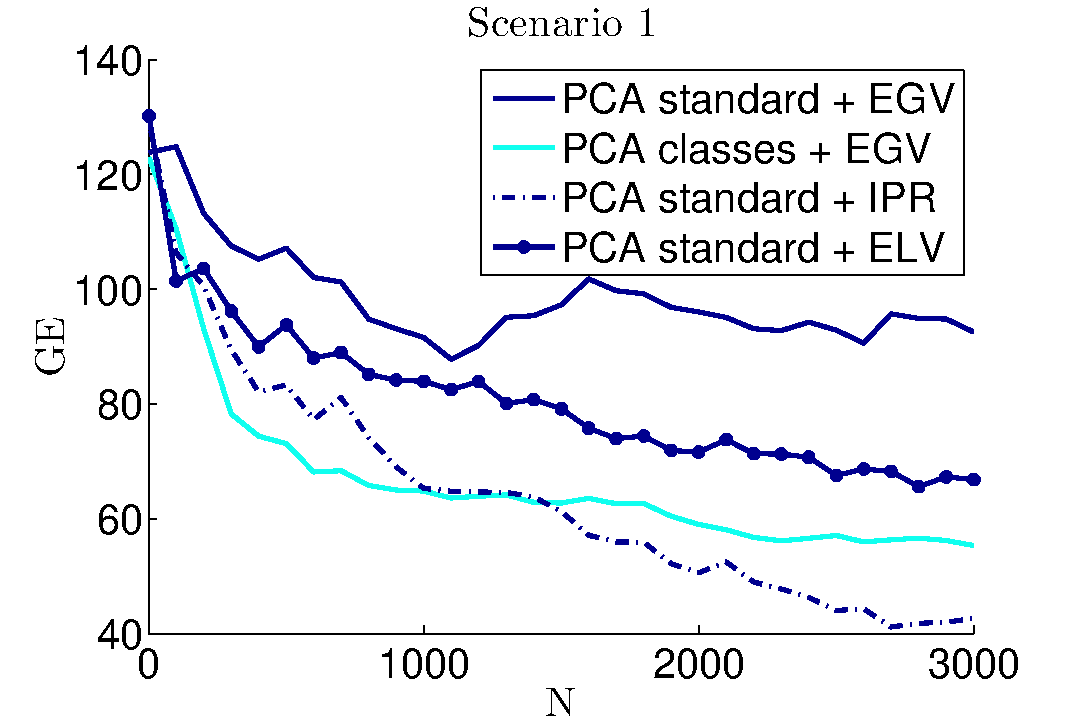
\includegraphics[width=0.4\textwidth]{figures/Criterion1.pdf}
%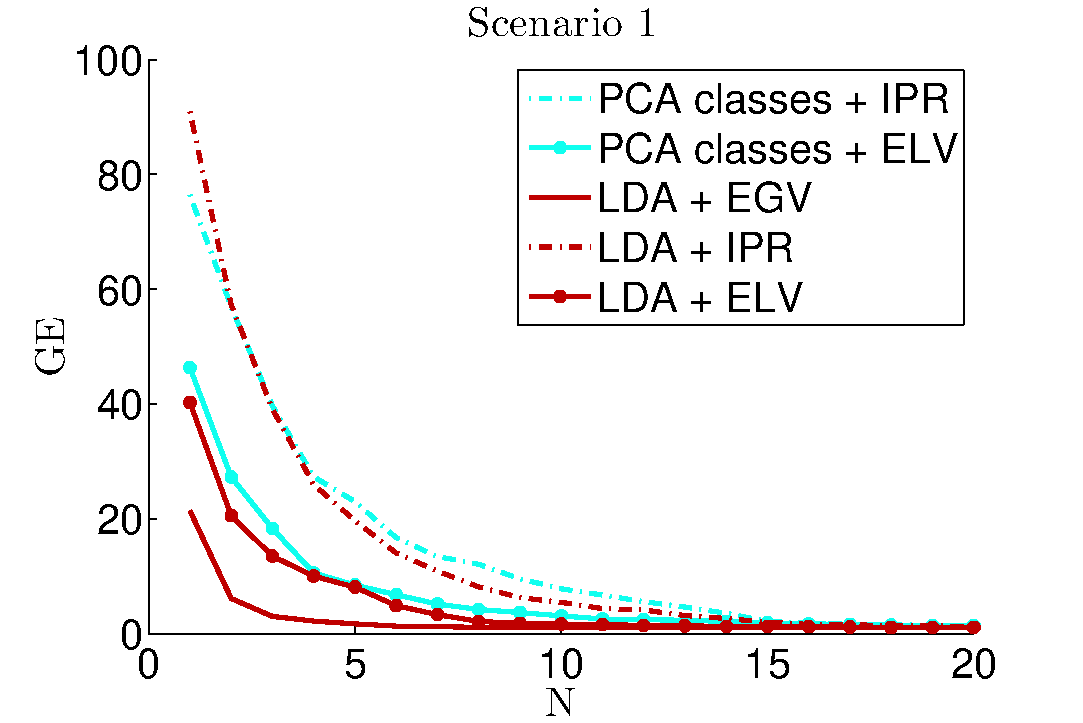
\includegraphics[width=0.4\textwidth]{figures/Criterion1Good.pdf}
%\caption{Guessing Entropy as function of the number of attack traces.}
%\end{figure}
%\vspace{-10pt}
%\begin{block}{Observations}
%\begin{itemize}
%\item LDA optimal (but more expensive)
%\item PCA close to LDA if equipped with ELV (and less expensive)
%\end{itemize}
%\end{block}
%
%\end{frame}
%
%\begin{frame}
%\vspace*{-2pt}
%\frametitle{Experimental results (minimizing $N_p$)}
%
%\vspace{-10pt}
%\begin{figure}
%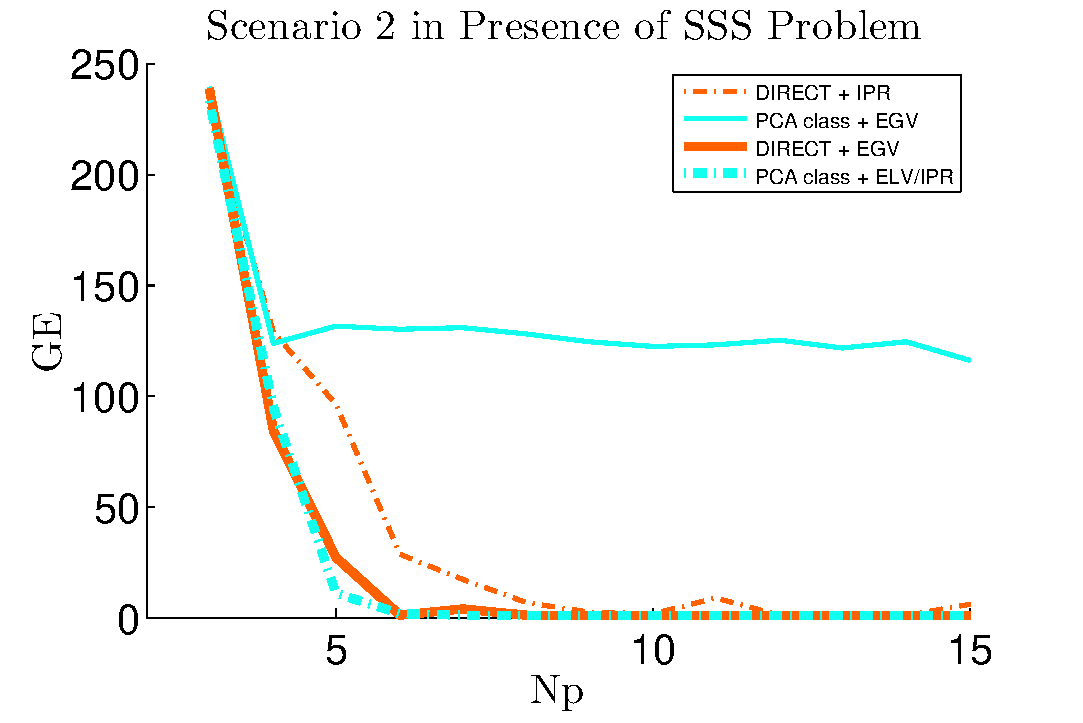
\includegraphics[width=0.4\textwidth]{figures/SSS.pdf}
%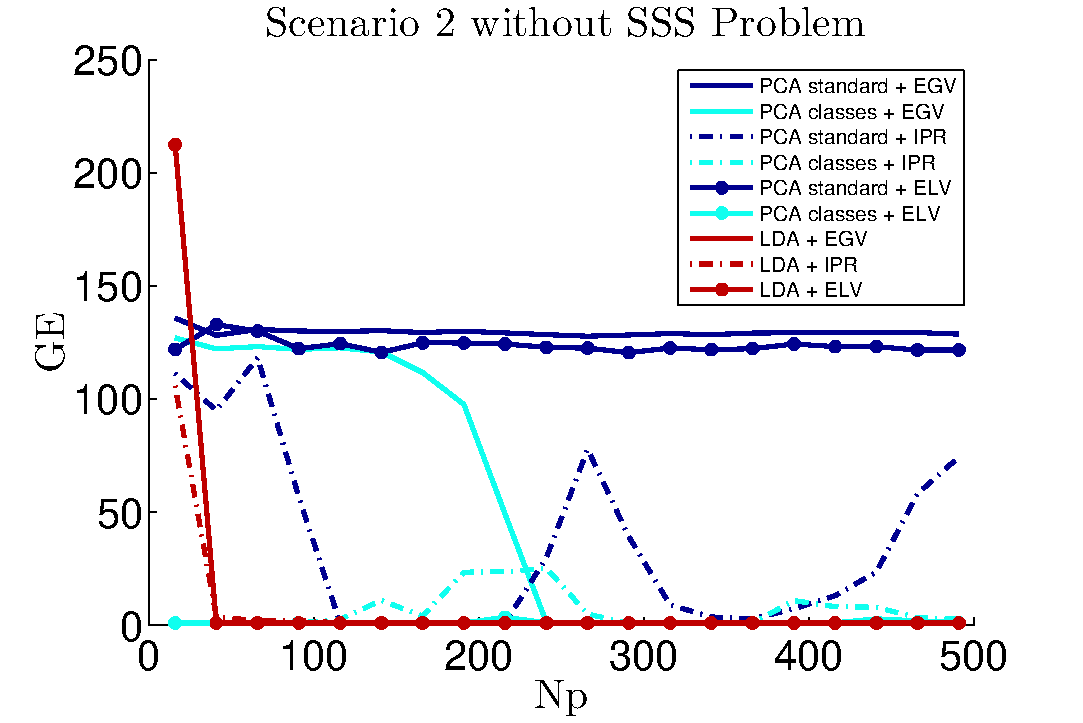
\includegraphics[width=0.4\textwidth]{figures/Criterion2notSSS.pdf}
%\caption{Guessing Entropy as function of the number of profiling traces.}
%\end{figure}
%
%\begin{block}{Observations}
%\begin{itemize}
%\item if LDA unavailable: PCA$+$ELV best alternative
%\item if LDA available: its efficiency is affected by the lack of profiling traces, PCA $+$ ELV keeps better
%\end{itemize}
%\end{block}
%
%\end{frame}